%\documentclass[10pt,twocolumn,letterpaper,draft]{article}
\documentclass[10pt,letterpaper]{ctexart}

\usepackage{cvpr}
% \usepackage{epsfig}
\usepackage{graphicx}
\usepackage{amsmath}
\usepackage{amssymb}
% \usepackage{color}
\usepackage{subfigure}
\usepackage{algorithm}
\usepackage{algorithmicx}
\usepackage{algpseudocode}
\usepackage{listings}

\renewcommand{\labelenumi}{\alph{enumi}.} % Make numbering in the enumerate environment by letter rather than number (e.g. section 6)
\floatname{algorithm}{算法}
\renewcommand{\algorithmicrequire}{\textbf{输入:}}
\renewcommand{\algorithmicensure}{\textbf{输出:}}

\usepackage{enumitem}
\setenumerate[1]{itemsep=0pt,partopsep=0pt,parsep=\parskip,topsep=5pt}
\setitemize[1]{itemsep=0pt,partopsep=0pt,parsep=\parskip,topsep=5pt}
\setdescription{itemsep=0pt,partopsep=0pt,parsep=\parskip,topsep=5pt}

% Include other packages here, before hyperref.

% If you comment hyperref and then uncomment it, you should delete
% egpaper.aux before re-running latex.  (Or just hit 'q' on the first latex
% run, let it finish, and you should be clear).
\usepackage[pagebackref=true,breaklinks=true,letterpaper=true,colorlinks,bookmarks=false]{hyperref}


\cvprfinalcopy % *** Uncomment this line for the final submission

\def\cvprPaperID{159} % *** Enter the CVPR Paper ID here
\def\httilde{\mbox{\tt\raisebox{-.5ex}{\symbol{126}}}}

\newcommand{\mypara}[1]{\paragraph{#1.}}

\graphicspath{{figures/}}

% Pages are numbered in submission mode, and unnumbered in camera-ready
%\ifcvprfinal\pagestyle{empty}\fi
\setcounter{page}{1}


%\begin{CJK*}{GBK}{song}

\newcommand{\figref}[1]{图\ref{#1}}
\newcommand{\tabref}[1]{表\ref{#1}}
\newcommand{\equref}[1]{式\ref{#1}}
\newcommand{\secref}[1]{第\ref{#1}节}

\ctexset{
  section={
          name={,、},
          number={\chinese{section}},
          format={\heiti},
          beforeskip={0.1ex},
          afterskip={0.1ex},
          aftername={\nobreak},
          indent={\parindent},
          },
}
\usepackage{zhnumber}

\newcommand\zhsubsec[1]{{% 中文小节
\bfseries{
\stepcounter{subsection}(\zhnum{subsection}){#1}}
\vspace{0.1pt}%
}}

%%%%%%%%% TITLE
\begin{document}
\pagestyle{plain}
\title{
    \begin{center}
        \phantom{Start!}
    	  \vspace{2cm}
        \center{\zihao{1} 中山大学数据科学与计算机学院}
        \center{\zihao{2} 《高性能程序设计基础》实验6}
        \center{(2018-2019学年秋季学期)}
    \end{center}
}
\maketitle

\begin{center}
    \setlength{\baselineskip}{40pt}
    \vspace{1cm}
    \zihao{-2}
    \center{
        \begin{tabular}{cc}
      	学\qquad 号:& \underline{~~~~~~16337113~~~~~~}  \\
      	姓\qquad 名:& \underline{~~~~~~~劳马东~~~~~~~}  \\
        教学班级:   & \underline{~~~~~教务2班~~~~~}  \\
      	专\qquad 业:& \underline{~~~~~~~~~超算~~~~~~~~}  \\
      	\end{tabular}
    }
\end{center}
\pagebreak

%%%%%%%%% BODY TEXT %%%%%%%%%%%%
% \begin{enumerate}[itemindent=2.5em,label=\arabic*、]
% \end{enumerate}

% \begin{algorithm}
%     \begin{algorithmic}[1] %每行显示行号
%         \Function {$TreeSearch$}{$Frontier, Successors,
%         \EndFunction
%     \end{algorithmic}
% \end{algorithm}

% \begin{figure}[h]
%   \centering
%   \subfigure[Completeness]{
%   \includegraphics[width=0.4\textwidth]{dfs-1.png}
%   \label{fig:dfs-1}}
% \end{figure}

\section{实验题目}
\begin{enumerate}[itemindent=1.5em,label=\arabic*、]
\item 完成正则采样排序PSRS的MPI算法;
\item 按要求使用MPI集合通信。
\end{enumerate}

\section{实验过程}
\zhsubsec{元素划分与采样}
\begin{enumerate}[itemindent=2.5em,label=\arabic*、]
\item 本地数据排序
\item 按进程数N等间隔采样
\end{enumerate}


\begin{figure}[h]
  \centering
  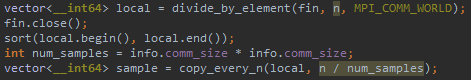
\includegraphics[width=0.8\textwidth]{step1.PNG}
  \label{fig:step-1}
  \caption{第一步}
\end{figure}

\zhsubsec{划分主元}
\begin{enumerate}[itemindent=2.5em,label=\arabic*、]
\item 收集样本
\par \qquad 一个进程收集样本(用MPI集合通信)并对所有样本进行排序;
\item 采样获得主元
\par \qquad 按进程数N对全体样本等间隔采样;
散发最终样本(用MPI集合通信),即主元。
\end{enumerate}

\begin{figure}[h]
  \centering
  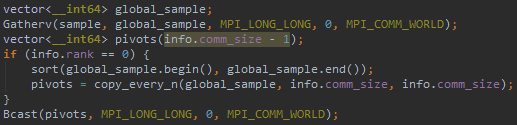
\includegraphics[width=0.8\textwidth]{step2.PNG}
  \label{fig:step-2}
  \caption{第二步}
\end{figure}

\zhsubsec{交换数据}
\begin{enumerate}[itemindent=2.5em,label=\arabic*、]
\item 本地数据分块
\item 全交互
\par \qquad
\end{enumerate}

\begin{figure}[h]
  \centering
  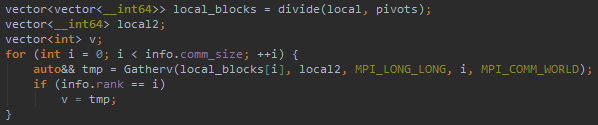
\includegraphics[width=0.9\textwidth]{step3.PNG}
  \label{fig:step-3}
  \caption{第三步}
\end{figure}

\zhsubsec{归并排序}

\begin{figure}[h]
  \centering
  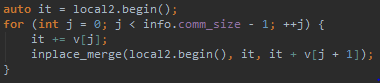
\includegraphics[width=0.6\textwidth]{step4.PNG}
  \label{fig:step-4}
  \caption{第四步}
\end{figure}

\section{关键代码}
\section{实验结果及分析}
\begin{enumerate}
    \item 正确性验证
    \item 评测指标展示及分析
\end{enumerate}

\end{document}
